\documentclass[../TST.tex]{subfiles}
\begin{document}
\begin{large}
	\textbf{Short Exam 2}
\end{large}

\begin{sproblem}
A monochromatic ($\lambda=\qty{500}{nm}$) point source $S$ illuminates a rectangular mirror $O$ which rotates at a frequency of $\nu=\qty{16}{Hz}$. The distance between the source and the mirror is $L=\qty{100}{m}$. The reflected light is sent to a detector $D$ of negligible size located close to the source. The mirror rotates about an axis that lies in the plane of the mirror and is perpendicular to the plane in which the reflected ray moves. You can assume that the source, the detector, and the mirror are collinear. Accounting for diffraction, find the duration $\Delta t$ of the light pulse registered by the detector. What is the width $a$ of the mirror that minimises $\Delta t$? What is the value of $\Delta t$ then? The height of the mirror is much larger than $a$.
\begin{figure}[h]
\centering
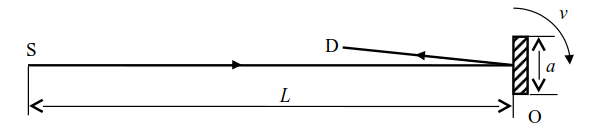
\includegraphics[width=0.8\textwidth]{fig/2007_l2.png}
\caption{}
\label{mirr}
\end{figure}
\end{sproblem}

\ifprob \else
	\begin{solution} There are two factors to consider here. The first is related to ray optics. The mirror will get to rotate by some small angle $\theta_g$ starting from the position in the figure, after which no points on the mirror will reflect anything towards the detector\footnote{In the original problem statement, the detector is said to be near the mirror rather than the source. But in that case you would definitely need the exact distance between the mirror and the detector, which isn't specified. I also have it on good authority that the answer for the optimal $a$ is indeed $\sqrt{\lambda L}$, which can't be obtained unless the detector is actually near the source.}.
\end{solution}
\begin{center}
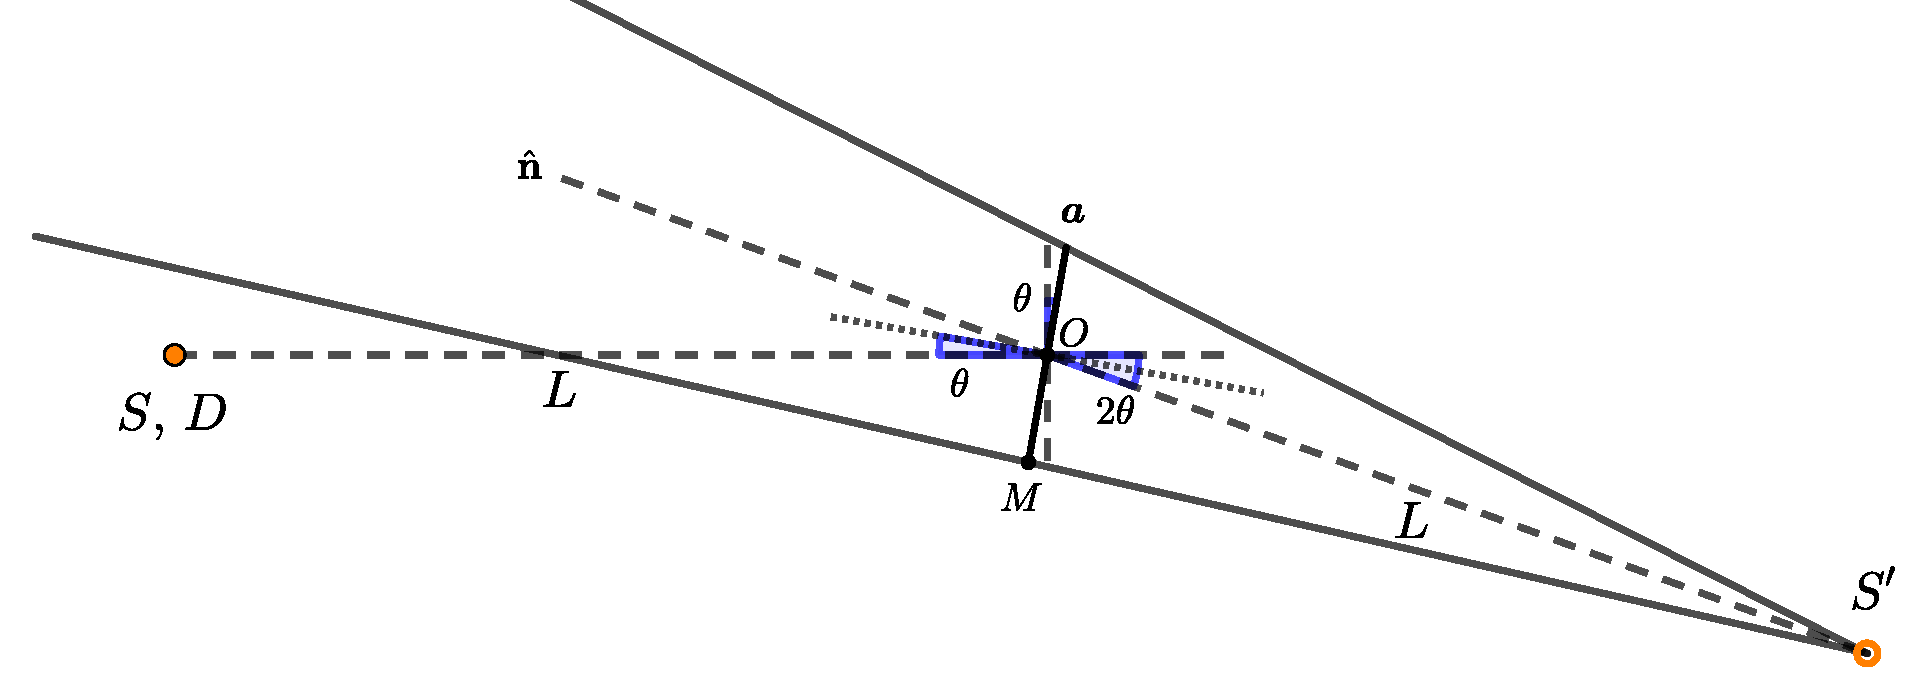
\includegraphics[width=0.9\textwidth]{fig/a2007_l2.pdf}
\end{center}
Referring to the figure, this happens when the cone of the rays emanating from the image $S'$ no longer includes the source $S$. This is the same as requiring $\angle OSS' \geq \angle OSM$. Given that $SS'\perp OM$, we have $\angle OSS'=\theta$, and since the mirror's tilt is small, we can write $\angle OSM = \frac{a/2}{L}$. Thus $\theta_g=\frac{a}{2L}$.\\[5pt]
We'll also need to account for diffraction. The reflection from the mirror isn't perfect, and it will essentially act as an obstacle of size $a$ which creates a diffraction pattern centered in the direction of the reflected ray $\hat{\mathbf{n}}$. The angular width of the central maximum of the pattern as seen from the mirror is $\frac{2\lambda}{a}$, with $\frac{\lambda}{a}$ on each side. The light within the maximum will land on the detector even after the detector goes out of range for the geometrically reflected rays. This will cease after an additional rotation of $\theta_d$, such that $\angle SON = 2\theta_d = \frac{\lambda}{a}$. In total, the mirror rotates by $\theta_g+\theta_d= \frac{a}{2L}+\frac{\lambda}{2a}$ until the end of the pulse. The total length of the pulse corresponds to twice that value as the detector is accessible from before the mirror is vertical. Thus,
\begin{equation*}
	\Delta t = \frac{2(\theta_g+\theta_d)}{\omega}= \boxed{\frac{(a/L)+(\lambda/a)}{2\pi\nu}.}
\end{equation*}
To find the minimum of $\Delta t$, we set the derivative with respect to $a$ to zero, whereby
\begin{equation*}
	\frac{1}{L}-\frac{\lambda}{a^2}=0 \quad\Rightarrow\quad \boxed{a=\sqrt{\lambda L}=\qty{7.1}{mm}.}
\end{equation*}
Returning to the expression for $\Delta t$, we have
\begin{equation*}
 \boxed{\Delta t = \frac{1}{\pi\nu}\sqrt{\frac{\lambda}{L}}=\qty{1.4e-6}{s}.}
\end{equation*}

\fi
\ifprob 
	\clearpage
\else 
	\vspace*{5mm}
\fi
\end{document}

